\documentclass[12pt,spanish]{article}
\usepackage[spanish]{babel}
\usepackage{graphicx}
\usepackage{color}
\usepackage{xcolor}
\usepackage{colortbl}
\usepackage{amsthm,thmtools}
\usepackage{multirow}
\usepackage{amsmath}
\usepackage{subcaption}
\usepackage{adjustbox}
\usepackage{multirow}
\usepackage[hidelinks]{hyperref}
\usepackage{caption}
\usepackage{amsthm}
\usepackage{multicol}
\usepackage{float}
\usepackage{amsfonts}
\usepackage{titling}
\usepackage{soul}
\usepackage{listings}
\usepackage{mathtools}
\usepackage{amssymb}
\usepackage{amsfonts}
\usepackage{array}
\usepackage[framemethod=tikz]{mdframed}

\graphicspath{ {../img/}}
\selectlanguage{spanish}
\usepackage[utf8]{inputenc}
\usepackage{graphicx}
\usepackage[a4paper,left=3cm,right=2cm,top=2.5cm,bottom=2.5cm]{geometry}

\newenvironment{solution}{
	\par
	\textbf{Solución}
	\par
	\begin{center}
}
{
	\end{center}
}


\title{Ingeniería de Servidores}
\setlength{\droptitle}{10em}
\author{Carlos Sánchez Páez}

\makeindex
\begin{document}
\definecolor{light-gray}{gray}{0.95}
\lstset{columns=fullflexible,basicstyle=\ttfamily}
\surroundwithmdframed[
  hidealllines=true,
  backgroundcolor=light-gray,
  innerleftmargin=0pt,
  innertopmargin=0pt,
  innerbottommargin=0pt]{lstlisting}


\begin{titlepage}

 \newlength{\centeroffset}
 \setlength{\centeroffset}{-0.5\oddsidemargin}
 \addtolength{\centeroffset}{0.5\evensidemargin}
 \thispagestyle{empty}

 \noindent\hspace*{\centeroffset}
 \begin{minipage}{\textwidth}

  \centering
  
\includegraphics[width=0.9\textwidth]{logo_ugr.jpg}\\[1.4cm]

  \textsc{ \Large Modelos de Computación\\[0.2cm]}
  \textsc{GRADO EN INGENIERÍA INFORMÁTICA}\\[1cm]

  {\Huge\bfseries Preguntas de examen resueltas\\}
 \end{minipage}

 \vspace{1.5cm}
 \noindent\hspace*{\centeroffset}
 \begin{minipage}{\textwidth}
  \centering

  \textbf{Autor}\\ {Carlos Sánchez Páez}\\[4ex]
  
\includegraphics[width=0.4\textwidth]{etsiit_logo.png}\\[0.1cm]
  \vspace{1.5cm}
  
\includegraphics[width=0.5\textwidth]{decsai.jpg}\\[0.1cm]
  \vspace{1cm}
  \textsc{Escuela Técnica Superior de Ingenierías Informática y de Telecomunicación}\\
  \vspace{1cm}
  \textsc{Curso 2019-2020}
 \end{minipage}
\end{titlepage}
\thispagestyle{empty}
\newpage

\begin{enumerate}
	\item Determinar si la gramática $G=(\{S,A,B\},\{a,b,c,d\},P,S)$ donde P es el conjunto de reglas de producción:
	\[
		S \implies AB ; A \implies Ab ; A \implies a ; B \implies cB ; B \implies d
	\]
	genera un lenguaje de tipo 3.
	\begin{solution}
		Comenzamos a generar:
		\begin{gather*}
			S \implies AB \xRightarrow[A \implies Ab]{} AbB \xRightarrow[A \implies Ab]{} AbbB \xRightarrow[...]{} Ab^iB \xRightarrow[B \implies cB]{} Ab^icB \\ \xRightarrow[...]{} Ab^ic^jB \xRightarrow[A \implies a]{} ab^ic^jB \xRightarrow[B \implies d]{} ab^ic^jd
		\end{gather*}
		Vemos que generamos el lenguaje ${ab^ic^jd}$, que también se puede generar mediante la siguiente gramática:
		\[
			S \implies aB ; B \implies bB ; B \implies C ; C \implies cC ; C \implies d
		\]
		Como la gramática es de tipo 3 (sólo hay como máximo una variable a la derecha en todas las producciones), el lenguaje también lo es.
	\end{solution}

	\item Diseñar una máquina de estados que calcule el complemento a dos de un número binario.

	\begin{solution}
	El complemento a dos de un número binario se calcula obteniendo su complemento a uno y sumándole uno. Veamos algunos ejemplos:
	\begin{itemize}
		\item $C_2$(\textcolor{red}{1}\textcolor{blue}{100})=$C_1$(1100)+1=0011+1=\textcolor{red}{0}\textcolor{blue}{100}
		\item $C_2$(\textcolor{red}{11}\textcolor{blue}{10})=$C_1$(1110)+1=0001+1=\textcolor{red}{00}\textcolor{blue}{10}
		\item $C_2$(\textcolor{red}{11101}\textcolor{blue}{100})=$C_1$(11101100)+1=00010011+1=\textcolor{red}{00010}\textcolor{blue}{100}
	\end{itemize}
	Tras realizar varias operaciones nos damos cuenta de que existe una codificación que se mantiene:
	\begin{enumerate}
		\item Comenzamos leyendo el número de derecha a izquierda y escribimos lo que leemos en la salida (también de derecha a izquierda).
		\item Cuando encontremos el primer 1 lo escribimos en la cinta y a partir de ahí escribimos el complemento a uno del número que leamos (cambiamos 0 por 1 y viceversa).
	\end{enumerate}
	\newpage
	Esta codificación se puede expresar mediante una máquina de \textit{Mealy}:
	\begin{itemize}
		\item La cabeza lectora y escritora se desplazará de derecha a izquierda.
		\item Estados
			\begin{itemize}
				\item $q_0$: todavía no he leído el primer 1. Si leo 0, escribo 0 y me mantengo. Si leo 1, paso al estado $q_1$ y escribo 1.
				\item $q_1$: ya he leído el primer 1. Ahora debo aplicar el complemento a 1 (si leo 1 escribo 0 y viceversa). En ambos casos me mantengo.
			\end{itemize}
		Es decir, la máquina sería la siguiente:
			\begin{figure}[H]
				\centering
				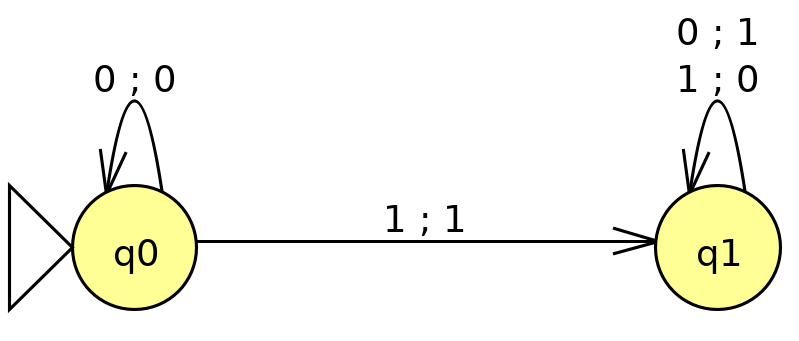
\includegraphics{ej2.png}
			\end{figure}
	\end{itemize}

	\end{solution}
	\item Si es posible, construir un autómata finito para el siguiente lenguaje:
	\[
		L=\{pcp^{-1} : p \in \{0,1\}^{*}\}
	\]
	En caso contrario, demostrar que no existe dicho autómata finito.

	\begin{solution}
		Para resolver este problema emplearemos el lema de bombeo. De un primer vistazo podemos ver que el lenguaje no es regular, ya que la relación sintáctica establecida (capicúa) es bastante fuerte.
		\begin{itemize}
			\item Suponemos que el lenguaje es regular, por lo que debe satisfacer el lema de bombeo.
			\item Comienzo eligiendo una cadena $z \in L$, por ejemplo, $z=0^nc0^n$. El lema de bombeo dice que $\exists n \in \mathbb{N} : z=uvw$.
			\item Comienzo a determinar el valor de u, v y w. Como la primera condición nos dice que $|uv| \leq n$, $uv$ debe ser una parte de $0^n$ (si fuera más no se cumpliría la condición). En este punto podemos determinar que $\boldsymbol{w=0^{n-k}c0^n}$ tal que $k<n \in \mathbb{N}$.
			\item La segunda condición nos dice que $\boldsymbol{|v| \geq 1}$, por lo que $\boldsymbol{v=0^l : l \geq 1$ y $u=0^{k-l}}$.
			Por ahora tenemos que $\boldsymbol{z=0^nc0^n=uvw=0^{k-l}0^l0^{n-k}c0^n}$.
			\item Ahora intentaremos buscar la contradicción bombeando, de forma que se incumpla que $\forall i \in \mathbb{N} : uv^iw \in L$. Para $i=0$:
			\[
				uv^0w=0^{k-l}0^{n-k}c0^n=0^{\pmb{n-l}}c0^{\pmb{n}} \notin L
			\]
			(el resultado tiene un número distinto de ceros a cada lado de $c$).\\
			Por tanto, queda demostrado que no existe un autómata finito para el lenguaje propuesto.
		\end{itemize}
	\end{solution}

	\item Construir un autómata con pila que acepte palíndromos de longitud par e impar.
	\begin{solution}
		El lenguaje que debe ser aceptado es $L=\{u \in \{0,1\}^{*} : u=u^{-1}\}$.\\
		Tendremos dos estados y tres símbolos:
		\begin{itemize}
			\item Estados
				\begin{itemize}
					\item $q_1$ cuando estemos apilando.
					\item $q_2$ cuando estemos desapilando.
			\end{itemize}
			\item Símbolos
			\begin{itemize}
				\item $Z$. Símbolo de fondo de pila.
				\item $B$. Recuerda que lo último introducido fue un 0.
				\item $G$. Recuerda que lo último introducido fue un 1.
		\end{itemize}
	\end{itemize}
	La dinámica sería leer un carácter de la cinta de entrada y meter en la pila el símbolo correspondiente. Cuando lleguemos a la mitad del palíndromo, deberemos desapilar. Si la pila queda vacía al terminar la lectura, aceptaremos la cadena.
	Nuestro autómata sería el siguiente:
		\begin{figure}[H]
			\centering
			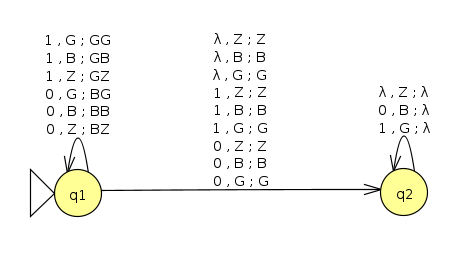
\includegraphics{ej4.png}
		\end{figure}
	\end{solution}
\end{enumerate}


\end{document}
